% Motivation: State assumption. Some way to model these planes in 3D and its transformation. We have some information. Inform what all restrictions we put. And why it is enough for us. No camera properties required. 
% Formulation: 
% Solution

In this thesis (Chapter \ref{ch:front}), we model face as a combination of planes in 3D. For example, consider the region
formed by the polygon with the end points as nose tip, point exactly between the eyes and bottom right
end of the nose. This region can be approximated to be a plane in 3D. We use a fiducial detector to 
find the key points on the face and triangulate to form various planes. The defined planes would undergo
transformations to achieve certain goal. The transformation of the defined planes would involve translation, 
rotations and scaling. This section provides mathematical formulation to address the various aspects of 
handling transformations of planes.

We use homogeneous notation for representing points as it can address the most generic projective 
transformations. Homogeneous representation of a 2D point $(x, y)$ in Euclidean space is represented as 
as a $3$ dimensional vector by adding a final coordinate of $1$, $(x, y, 1)^T$. A planar projective 
transformation of $3$ dimensional vector by a non-singular $3 \times 3$ matrix is represented by,

% \begin{equation}
% \left(
% \right)
% \end{equation}
\[
\begin{bmatrix}
x_1^{\prime} \\
x_2^{\prime} \\
x_3^{\prime} 
\end{bmatrix}
=
\begin{bmatrix}
h_{11} & h_{12} & h_{13} \\
h_{21} & h_{22} & h_{23} \\
h_{31} & h_{32} & h_{33} 
\end{bmatrix}
\begin{bmatrix}
x_1 \\
x_2 \\
x_3 
\end{bmatrix}
\label{eqn:homogenous}
\]

Based on the in-variances in properties of transformations, there are $4$ sub groups under projective 
transformations. They are isometrics, similarity transformations, affine transformations and projective
transformations. 

Isometric transformation is composition of just translation and rotation. Here the length 
(the distance between two points), angle (between two lines) and area is preserved. Similarity transformations
preserves the form and is composed of isometric scaling along with translation and rotation. In-variances
include angle, parallelity, ratio of lengths. Both isometrics and similarity transformations require two
point correspondences to compute transformation matrix. Affine transformation is a non-singular linear
transformation followed by a translation which has $6$ degrees of freedom and can be thought of as a 
combination of rotations and non-isotropic scalings along with translation. It requires $3$ point 
correspondences to compute the transformation matrix. In this case, parallel lines are preserved along with the
ratio of lengths of parallel line segments and ratio of areas. And finally the most generalized projective
transformation has $8$ degree of freedom and would require $4$ point correspondences to compute the 
transformation matrix. 

\begin{figure}
    \centering
    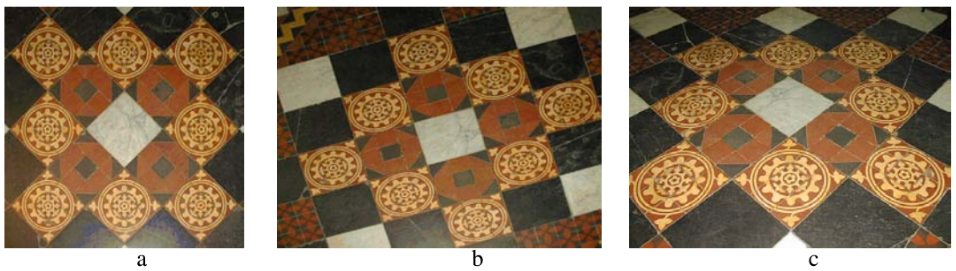
\includegraphics[width=6in, height=1.8in]{concepts/figures/affine_transformation.png}
    \caption{Pictorial representation of various transformations. (\textit{a}) \textbf{Similarity:} Observe the patterns preserved such as circular pattern, square shaped tiles, parallel and perpendicular lines.
    (\textit{b}) \textbf{Affine:} In this case, circles are imaged as ellipses, orthogonal lines are no more orthogonal, but the parallel lines are
    preserved. (\textit{c}) \textbf{Projective:} Area of tiles closer to camera is larger than the ones away and parallel world lines are converging. Image courtesy: Multiple View Geometry in Computer Vision\cite{Hartley2004}}
    \label{fig:affine_transformation}
\end{figure}

In this thesis, we consider affine transformation to model the planes on the face images. Since we triangulate
regions on the face image using the face fiducial detector, we have $3$ point correspondences to model the
corresponding planes between any two faces.
